\section{Methods}
\label{section:methods}
\subsection{Background on Reddit conversations}
Building on the brief descriptions in the previous sections, here we provide a more detailed background of Reddit conversations: In most forum based platforms such as reddit,  users interact in a nested dialogue fashion, where an Original Poster or $OP$ posts content called a Root Post or $RP$ to start  a new discussion thread. This thread is then open for comments by all the community users. In case of Reddit, such a community is called a Subreddit. Subreddits like SuicideWatch consist of a moderated collection of posts from users who subscribe to that community or subreddit. These users may post new threads onto the subreddit as long as the post follows the subreddit rules. Enforcement of these rules is the responsibility of the moderators. %The user who starts a thread is called the Original Poster or \textbf{OP} and the headlining post which the $OP$ begins with is called the Root Post or $RP$. 

\subsection{Datasets} \label{sec:data}
The focus our work is the subreddit r/SuicideWatch. We study this using a seed dataset~\cite{gkotsis2017characterisation}, that consists of root posts from the subreddit r/SuicideWatch. Building on this dataset, acquire the entire thread structure of all the root posts in the data by recursively obtaining all replies to the root posts, replies to those replies and so on, until we reach posts which do not have any further replies. This results in acquisition of 50,754 threads from SuicideWatch (SW). To obtain a baseline of similar size for comparison purposes, we crawl the entire conversation threads of posts that appear on the front page of Reddit.com  for 2 weeks,  accumulating a second corpus (FP) of 49,773 reddit threads in the process. 
%
The two conversation datasets from r/SuicideWatch and Frontpage are very similar in terms of common summary statistics such as Degree distributions (see Appendix Fig.~\ref{fig:degdist}). 
Owing to the long tailed nature of the datasets, we perform our analysis on threads  which have at least 5 posts in addition to the root post.
We further clean the data, by removing threads where the root author has deleted their user account, which is a common practice to preserve anonymity in more controversial posts. The resulting dataset has 10,527 threads in SW and 11,070 threads in the baseline (FP). 

\begin{figure}
    \centering
    \subfloat[]{
        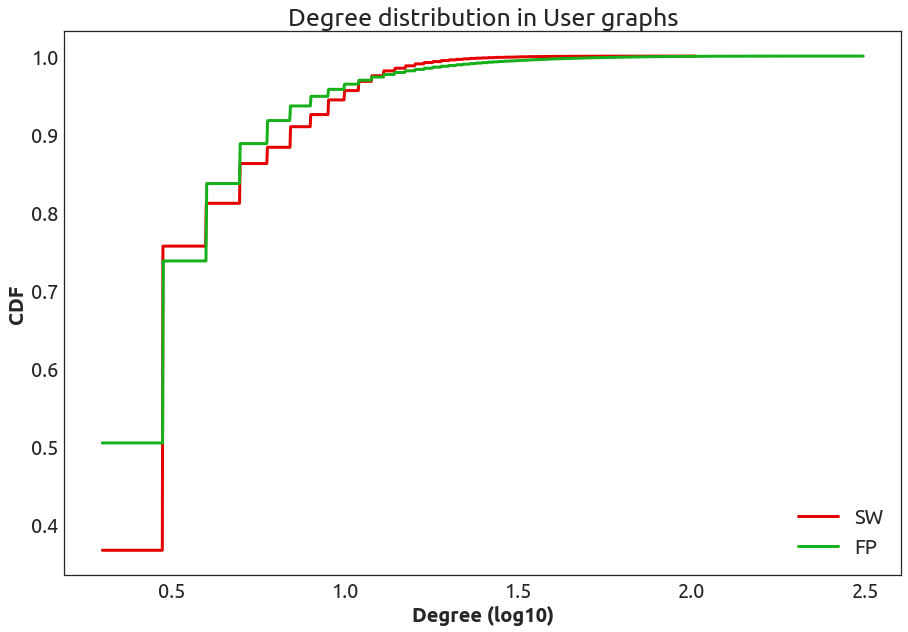
\includegraphics[width=0.25\textwidth ]{Figures/V1/UserDegDist.png}
        \label{fig:degUgraph}
    }
    \subfloat[]{
        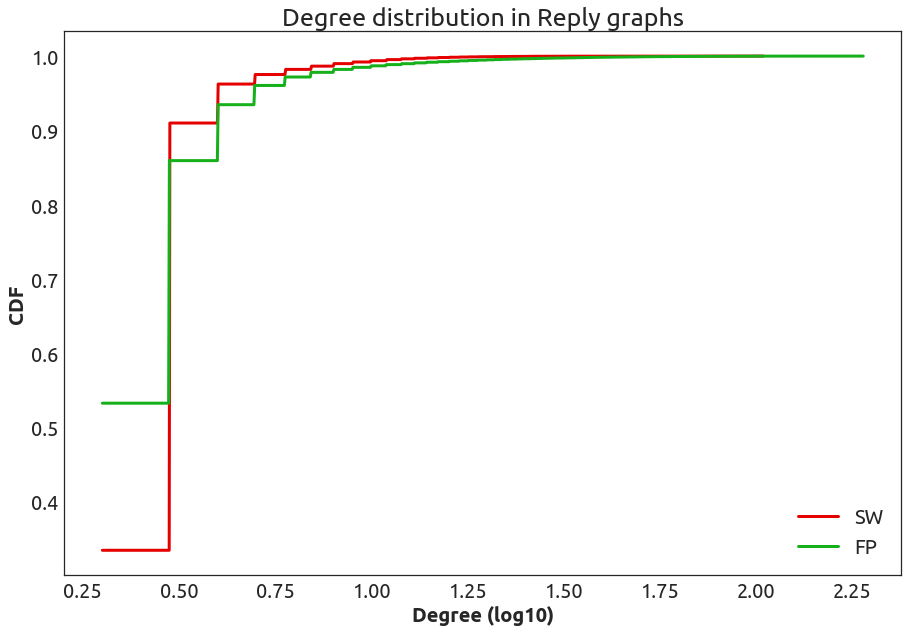
\includegraphics[width=0.25\linewidth]{Figures/V1/ReplyDegDist.png}
        \label{fig:degRgraph}
    }\caption{Degree distributions  (a) User Graph and (b) Reply Graphs in FP and SW, showing that the two datasets are comparable.}
    \label{fig:degdist}
\end{figure}

\subsection{Abstractions} \label{sec:abstractions}
To understand the dynamics of supportive conversations, develop two abstractions: 
\subsubsection{Reply Graphs} \label{sec:reply_graphs}
The first abstraction mimics directly the structure of conversation threads on Reddit with an abstraction we term as \textit{reply graphs}, and denote as $R = (P,E)$. The nodes $P$ consist of all the posts in the thread. The root post is labeled as $p_0 \in P$ and $k^{th}$ post in chronological order as $p_k \in P$. A directed edge ($p_i,p_j) \in E$ is drawn from $p_i$ to $p_j$ if $p_j$ is a reply to $p_i$. \ref{Fig:GraphExamples} (a) presents an example. Note that in platforms such as Reddit, where each response can only reply to one other post, reply graphs end up being reply \textit{trees}.
% %The weight of the edge $E_{ij}$ is found by calculating the cosine similarity between semantic vector $V_i$ for post $P_i$ and the semantic vector $V_j$ of post $P_j$.  This abstraction works well in modeling the conversational nature of these forums.  
% For convenience of the reader, we present a couple of example pairs from SW and Frontpage baseline datasets in Figure \ref{Fig:GraphExamples}

\subsubsection{User interaction Graphs} \label{sec:interaction_graphs}
The second abstraction, which we term \textit{user interaction graphs},  represents each thread as a directed graph $G = (V,E)$ where $V$ is the set of all users participating in a particular thread and a directed edge $(v_i, v_j) \in E$ is drawn between two users $v_i$ and $v_j$ if user $v_i$ responds to a post by user $v_j$. \ref{Fig:GraphExamples} (b) presents an example. Note that unlike reply trees, user interaction graphs of Reddit conversations can be full graphs, and may include cycles. %are the directed  edges which correspond to interactions between two users $V_i , V_j  \in V$. The weight of each directed edge $E_{ij}$ corresponds to the average of all the edge weights between $V_i , V_j  \in V$ in the corresponding reply graph $R\{P,E,W\}$ as described above. This means that each reply graph is then mapped to a User graphs where the nodes are users rather than posts. Another salient distinction between the two abstractions is that reply graphs resemble an n-ary tree and user graphs are directed cyclic graphs. 

% \subsubsection{Graph Edge weights}
% We use a popular word embedding method called \textit{Word2Vec} \cite{mikolov2013distributed} which learns representations of a set of words from a corpus of text, which in our case is the text from Suicide Watch and baseline fora. These representations can be used to extract text embedding vectors for each post which belong to a $N$ dimensional space $R^N$. These vectors are tested for their alignment using cosine distance in $R^N$, which from literature is shown to correspond to the semantic similarity in the textual space. %This method is quite popular and used in community based question answering\cite{mihaylov2016semanticz}, Medical semantic similarity \cite{de2014medical} and other medical informatics applications\cite{zhu2017semantic}.

% We first train two independent word2vec models on the Suicide watch and Front page post corpora. 
% We then extract the word embedding vectors for each post using Doc2Vec\cite{le2014distributed}, which extends the word embeddings to represent a whole document or paragraph. We extract these embedding vectors for each post in $R^N$ for all the posts across the complete hierarchy of threads. We then quantify the edge weights of each interaction amongst the reply tree as the cosine distance between the response post and the hierarchically higher post, to which the responder has posted to. This captures the semantic alignment between the hierarchically adjacent responses. 
% More formally, if user $V_i$ has responded with post $P_i$ to a post $P_j$ written by user $V_j$, we extract the word embedding in $R^N$ for both posts $P_i$ and $P_j$. If these embeddings are represented by $N$ dimensional vectors $\psi_i^N$ and $\psi_j^N$ then the edge weight for the edge $E_{ij}$ in the corresponding reply graph would be

% $$ W_{ij} = \frac{\psi_i^N . \psi_j^N}{\|\psi_i^N\|_2 \|\psi_j^N\|_2} $$


%This metric standardizes all edge weights between 0.0 and 1.0, 1.0 implying that the posts $P_i$ and $P_j$ are most aligned, and 0.0 implying the post have least semantic similarity. 
%This metric abstracts out the content of the post, in terms of semantics which can then be used as edge weights in the graph abstractions.

\subsection{Macroscopic graph metrics}
The abstractions are used to extract the following structural metrics from the conversation threads. These metrics are then used to validate structural differences between supportive conversations and generic casual conversations from our baseline set.%, and come up with a theory for links between supportive conversations and the structure of the conversation, if we find any.



\subsubsection{Responsiveness}
To understand the speed with which users in a subreddit (whether in SW or in other subreddits as represented in FP) respond to the $OP$ and each other,  we calculate differences between the posting times between consecutive response messages in a reply graph. We then compute the median response times per thread.


\subsubsection{Reciprocity}
Reciprocity measures the extent to which users' posts obtain responses, and is measured as the fraction of edges in the user graph that are bidirectional:
$$
U_{sym}=\frac{\textit{total number of bidirectional edges in a user graph}}{\textit{Total number of edges in the graph}}
$$

\subsubsection{OP Centrality} \label{sec:centrality}
Node centrality is a metric that measures how central a node is in a network. We study how central the OP is to a conversation thread by computing how often it lies on the shortest connecting paths between other pairs of nodes in the user interaction graph. Betweenness centrality is formally defined as 
$$
g(OP) = \sum_{s \neq v \neq t}\frac{\sigma_{st}(OP)}{\sigma_{st}}
$$
where $\sigma_{st}$ is the total number of shortest paths from node $s$ to node $t$ and $\sigma_{st}(OP)$ is the number of those paths that pass through $OP$. %To understand whether the thread starters ($OP$) have a special place in the network, we evaluate both centrality of the node corresponding to the $OP$, as well as median centrality across all the nodes in a user graph.


% \subsubsection{Semantic alignment} \label{sec:semantic_alignment}
% This metric quantifies the overall semantic alignment between response posts across a particular conversation thread. For any reply graph $R\{P,E\}$, we compute the median of all the edge weights calculated using the definition of semantic alignment 
% This metric quantifies the overall semantic alignment in a conversation. We also do the same calculation between responses to any post authored by the $OP$ to test whether responses to $OP$ demonstrate any special pattern of all alignment in supportive vs generic threads.

\subsubsection{Branching Factor}\label{sec:branching}
Branching factor is a metric that reflects the fanning out of a conversation as it evolves. To measure this on Reddit reply trees. we compute the average number of replies obtained by each post, i.e., the average in-degree of nodes in each reply graph. 
%how the node population increases as you go deeper into the reply graph. The branching factor is formally described by the formula 
% $$\tau = \frac{1}{D} \sum_{d = 0}^{D} \frac{1}{|N_d|} \sum_{n\in N_d}^{} \textit{InDeg}(n)$$
% where $D$ represents the maximum depth of a particular reply graph, $N_d$ represent the set of all nodes found at depth $d$ and $|N_d|$ represents the total number of nodes at depth $d$. $\textit{InDeg}(n)$ is the \textit{in-degree} of node $n$, i.e., represents total number of edges that terminate at node $n$.
% \ns{Is there a reason why you have to do this on a per depth basis, when you are just aggregating across all nodes? Isn't the double sum you have just the average indegree of all nodes?}


%Local properties: 
\subsection{Mesoscopic graph metrics: Anchored triadic motifs  } \label{sec:motif}
Network motifs are local sub-networks, typically of 2 or 3 nodes which are connected together. Such local patterns are highly useful in quantifying local interactions and the resulting macro structure of the network\cite{milo2002network}. They have been used in a variety of applications, from economics \cite{zhang2014dynamic} to cellular protein-protein interaction networks \cite{yeger2004network}. These local interaction patterns have been fundamental in the study of social structural processes\cite{faust20077}. They help social scientists quantify the type of hierarchies in the social network\cite{davis1967clustering,davis1967structure}. Hence, we turn to network motifs to characterize the local structure of the converstion threads. 
However, SW conversations shows clear distinctions between the users who respond to a call for help and the user/s who are asking for help (the $OP$). To accommodate this, we extend the concept of triadic motifs to create different variants of the same motif when the $OP$ is in different positions.

In conventional literature, the local interactions are measured through a census of 16 triadic motif patterns\cite{faust20077}, which cover all possible patterns of non-isomorphic triads which cannot be mapped or morphed into each other. In this method, there is no special treatment to any node, and position of all nodes is treated equally. To this, we introduce the notion of \textit{anchors}, or nodes with special importance, which in our case is the $OP$, the user who makes the initial post in the thread under consideration. 
By fixing a role for a node in a motif, each of the 16 triadic motifs as seen and developed in the field\cite{faust20077, holland1977method}, can be unravelled into 36 sub-variants of these motifs by varying the anchored node, as seen in Fig \ref{fig:motifs}. Each sub-variant is different from the other from the perspective of the anchored node. Some motifs yield three variants for each of the three positions that the $OP$ can be in. However, other motifs yield fewer variants, since two or more of the variants can be iso-morphic to each other even when the position of the $OP$ is distinguished.  Bataglej et.al's work\cite{Batagelj2001} developed a method for counting network motifs. We build on this and develop an efficient method for counting anchored network motifs. 
Each motif as seen in Figure \ref{fig:motifs} is named using the naming scheme  developed by Holland and Leinhardt\cite{holland1974statistical}. The first three numbers, follow a M-A-N pattern which signifies the number of "\textbf{M}utual" , "\textbf{A}symmetric" or "\textbf{N}ull" edges present in that particular triad. For example, the motif 030 has 0-Mutual(bi-directional), 3-Asymmetric(unidirectional) and 0-Null (disconnected) edges. There are some motifs with an added modifier letter (C-U-D-T) attached to further differentiate between different triad types with the same M-A-N pattern.
To this, we additionally attach a variant label (a, b or c) to distinguish the different anchored network motifs that result from the different positions of the $OP$.


To systematically understand the over or under expression of these anchored triadic motifs in the suicide watch community (SW), we use the user interaction graphs for the Front page (FP) baseline posts as a null model. We analyse 10,527 user interaction graphs from SW and 11,070 graphs from FP dataset.
We progressively select graphs with different sizes, i.e., graphs with differing number of users present in the interaction graphs. We bin both the FP and SW user interaction graphs as follows, based on the number of nodes interacting within a thread: 1 - 5, 6 - 10 , 11 - 15 , 16 - 20 , 21 - 25, 26 - 30, 31 - 35 and 36 - 40. The number of conversations that contain more than 40 unique users participating in the same conversation thread is extremely small in both SW and FP; hence we stop binning at this point.
Within each bin, we then perform a census, counting the number of occurrences of different anchored network motifs. 
Once the census is done, we calculate $Z_{scores}$ for the Suicide watch conversations, using FP conversations as the null model, to understand whether a given anchored network motif is over or under expressed in SW in relation to FP.


 %We do this by first progressively selecting bins, both from the $FP$ and $SW$ datasets. 
 
 We call the set of FrontPage and SuicideWatch graphs that belong to bin $b$ as $G^b_{FP}$ and $G^b_{SW}$ respectively. For a selected bin $b$, let $M$ graphs from $FP$ belong to $b$ and $N$ from $SW$ belong to $b$. We conduct the anchored motif census of the 36 motifs for both $G^b_{FP}$ and $G^b_{SW}$.  
To compute the null model, we require the mean ($\mu_{null}$) and standard deviation ($\sigma_{null}$) of the frequency distributions of all the 36 motifs found in the $G^b_{FP}$ graphs. This means we will have 36 values of ($\mu_{null}$) and ($\sigma_{null}$); one for each motif. We also compute the mean ($\mu_{SW}$) and standard deviation ($\sigma_{SW}$) for $SW$ dataset, and plot the means of $FP$ and $SW$ side by side as a comparison. The error bars represent standard errors ( $ e_{null} = \frac{\sigma_{null}}{\sqrt{M}}$ and $ e_{SW} = \frac{\sigma_{SW}}{\sqrt{N}}$). Plots of these mean frequencies for both datasets can be found in Figures \ref{fig:021U-a} -- \ref{fig:021C-c}.

Once we have the null model figures for the bin $b$ from $G^b_{FP}$ graphs, we  compare these with the $N$  graphs ($G^b_{SW}$) in order to compute the $Z_{score}$. For the $i^{th}$ motif, the score $Z_{i}$ is defined as 

$$Z_i = \frac{1}{N} \sum_{k=1}^{N} \frac{m_k^{SW} - \mu_{null}}{\sigma_{null}}$$ 

where $m_k^{SW}$ is the total number of the $i^{th}$ motif found in the $k^{th}$ graph in $G^b_{SW}$. We compute this $Z_{score}$ for all the 36 motifs across all the 7 bins. The trends in the value of this $Z_{score}$ are also plotted in Figure \ref{fig:motifs}. We consider a motif population as significant if the mean motif population goes above 10 for any of the 7 bins. We consider a motif over/under expressed if the Z-score is either greater than 1 or less than -1 for at least 1 bin. A motif which has significant mean population but has a Z-score between -1 and 1 is considered equally expressed. Figure \ref{fig:motifs} shows all the 8 motifs which are significant and over/under expressed, 
where as the measurements of the statistically insignificant motifs are included in the supplementary material.